\documentclass[twoside]{book}

% Packages required by doxygen
\usepackage{fixltx2e}
\usepackage{calc}
\usepackage{doxygen}
\usepackage[export]{adjustbox} % also loads graphicx
\usepackage{graphicx}
\usepackage[utf8]{inputenc}
\usepackage{makeidx}
\usepackage{multicol}
\usepackage{multirow}
\PassOptionsToPackage{warn}{textcomp}
\usepackage{textcomp}
\usepackage[nointegrals]{wasysym}
\usepackage[table]{xcolor}

% Font selection
\usepackage[T1]{fontenc}
\usepackage[scaled=.90]{helvet}
\usepackage{courier}
\usepackage{amssymb}
\usepackage{sectsty}
\renewcommand{\familydefault}{\sfdefault}
\allsectionsfont{%
  \fontseries{bc}\selectfont%
  \color{darkgray}%
}
\renewcommand{\DoxyLabelFont}{%
  \fontseries{bc}\selectfont%
  \color{darkgray}%
}
\newcommand{\+}{\discretionary{\mbox{\scriptsize$\hookleftarrow$}}{}{}}

% Page & text layout
\usepackage{geometry}
\geometry{%
  a4paper,%
  top=2.5cm,%
  bottom=2.5cm,%
  left=2.5cm,%
  right=2.5cm%
}
\tolerance=750
\hfuzz=15pt
\hbadness=750
\setlength{\emergencystretch}{15pt}
\setlength{\parindent}{0cm}
\setlength{\parskip}{3ex plus 2ex minus 2ex}
\makeatletter
\renewcommand{\paragraph}{%
  \@startsection{paragraph}{4}{0ex}{-1.0ex}{1.0ex}{%
    \normalfont\normalsize\bfseries\SS@parafont%
  }%
}
\renewcommand{\subparagraph}{%
  \@startsection{subparagraph}{5}{0ex}{-1.0ex}{1.0ex}{%
    \normalfont\normalsize\bfseries\SS@subparafont%
  }%
}
\makeatother

% Headers & footers
\usepackage{fancyhdr}
\pagestyle{fancyplain}
\fancyhead[LE]{\fancyplain{}{\bfseries\thepage}}
\fancyhead[CE]{\fancyplain{}{}}
\fancyhead[RE]{\fancyplain{}{\bfseries\leftmark}}
\fancyhead[LO]{\fancyplain{}{\bfseries\rightmark}}
\fancyhead[CO]{\fancyplain{}{}}
\fancyhead[RO]{\fancyplain{}{\bfseries\thepage}}
\fancyfoot[LE]{\fancyplain{}{}}
\fancyfoot[CE]{\fancyplain{}{}}
\fancyfoot[RE]{\fancyplain{}{\bfseries\scriptsize Generated by Doxygen }}
\fancyfoot[LO]{\fancyplain{}{\bfseries\scriptsize Generated by Doxygen }}
\fancyfoot[CO]{\fancyplain{}{}}
\fancyfoot[RO]{\fancyplain{}{}}
\renewcommand{\footrulewidth}{0.4pt}
\renewcommand{\chaptermark}[1]{%
  \markboth{#1}{}%
}
\renewcommand{\sectionmark}[1]{%
  \markright{\thesection\ #1}%
}

% Indices & bibliography
\usepackage{natbib}
\usepackage[titles]{tocloft}
\setcounter{tocdepth}{3}
\setcounter{secnumdepth}{5}
\makeindex

% Hyperlinks (required, but should be loaded last)
\usepackage{ifpdf}
\ifpdf
  \usepackage[pdftex,pagebackref=true]{hyperref}
\else
  \usepackage[ps2pdf,pagebackref=true]{hyperref}
\fi
\hypersetup{%
  colorlinks=true,%
  linkcolor=blue,%
  citecolor=blue,%
  unicode%
}

% Custom commands
\newcommand{\clearemptydoublepage}{%
  \newpage{\pagestyle{empty}\cleardoublepage}%
}

\usepackage{caption}
\captionsetup{labelsep=space,justification=centering,font={bf},singlelinecheck=off,skip=4pt,position=top}

%===== C O N T E N T S =====

\begin{document}

% Titlepage & ToC
\hypersetup{pageanchor=false,
             bookmarksnumbered=true,
             pdfencoding=unicode
            }
\pagenumbering{alph}
\begin{titlepage}
\vspace*{7cm}
\begin{center}%
{\Large elevator }\\
\vspace*{1cm}
{\large Generated by Doxygen 1.8.13}\\
\end{center}
\end{titlepage}
\clearemptydoublepage
\pagenumbering{roman}
\tableofcontents
\clearemptydoublepage
\pagenumbering{arabic}
\hypersetup{pageanchor=true}

%--- Begin generated contents ---
\chapter{Data Structure Index}
\section{Data Structures}
Here are the data structures with brief descriptions\+:\begin{DoxyCompactList}
\item\contentsline{section}{\hyperlink{structfsm__t}{fsm\+\_\+t} }{\pageref{structfsm__t}}{}
\end{DoxyCompactList}

\chapter{File Index}
\section{File List}
Here is a list of all documented files with brief descriptions\+:\begin{DoxyCompactList}
\item\contentsline{section}{source/{\bfseries fsm.\+c} }{\pageref{fsm_8c}}{}
\item\contentsline{section}{source/\hyperlink{fsm_8h}{fsm.\+h} \\*Finite state machine for an elevator }{\pageref{fsm_8h}}{}
\item\contentsline{section}{source/\hyperlink{hardware_8h}{hardware.\+h} \\*Driver for the elevator hardware }{\pageref{hardware_8h}}{}
\item\contentsline{section}{source/{\bfseries main.\+c} }{\pageref{main_8c}}{}
\item\contentsline{section}{source/{\bfseries queue.\+c} }{\pageref{queue_8c}}{}
\item\contentsline{section}{source/\hyperlink{queue_8h}{queue.\+h} \\*Elevator queue implementation }{\pageref{queue_8h}}{}
\item\contentsline{section}{source/{\bfseries timer.\+c} }{\pageref{timer_8c}}{}
\item\contentsline{section}{source/\hyperlink{timer_8h}{timer.\+h} \\*Implements a timer that times out in {\ttfamily T\+I\+M\+E\+R\+\_\+\+T\+I\+M\+E\+O\+U\+T\+\_\+\+S\+E\+C\+O\+N\+DS} seconds }{\pageref{timer_8h}}{}
\end{DoxyCompactList}

\chapter{Data Structure Documentation}
\hypertarget{structfsm__t}{}\section{fsm\+\_\+t Struct Reference}
\label{structfsm__t}\index{fsm\+\_\+t@{fsm\+\_\+t}}
\subsection*{Data Fields}
\begin{DoxyCompactItemize}
\item 
state\+\_\+function \hyperlink{structfsm__t_a712771896c61fba0983cdf9bb7c5aef3}{state}
\item 
fsm\+\_\+state\+\_\+t \hyperlink{structfsm__t_a2ee302f4baedf2779e08f3d0cba24ae1}{state\+\_\+name}
\item 
int \hyperlink{structfsm__t_a39d1b1b17a203c65eef47e1c20f81b2c}{current\+\_\+floor}
\item 
direction\+\_\+t \hyperlink{structfsm__t_a4a22f2e6606e51b6d83309023ac1b4fc}{direction}
\item 
relative\+\_\+position\+\_\+t \hyperlink{structfsm__t_ad6a67b3201e4002d25f058bb8bf9ffd5}{position}
\end{DoxyCompactItemize}


\subsection{Detailed Description}


Definition at line 32 of file fsm.\+c.



\subsection{Field Documentation}
\mbox{\Hypertarget{structfsm__t_a39d1b1b17a203c65eef47e1c20f81b2c}\label{structfsm__t_a39d1b1b17a203c65eef47e1c20f81b2c}} 
\index{fsm\+\_\+t@{fsm\+\_\+t}!current\+\_\+floor@{current\+\_\+floor}}
\index{current\+\_\+floor@{current\+\_\+floor}!fsm\+\_\+t@{fsm\+\_\+t}}
\subsubsection{\texorpdfstring{current\+\_\+floor}{current\_floor}}
{\footnotesize\ttfamily int fsm\+\_\+t\+::current\+\_\+floor}

Current floor number of elevator 

Definition at line 35 of file fsm.\+c.

\mbox{\Hypertarget{structfsm__t_a4a22f2e6606e51b6d83309023ac1b4fc}\label{structfsm__t_a4a22f2e6606e51b6d83309023ac1b4fc}} 
\index{fsm\+\_\+t@{fsm\+\_\+t}!direction@{direction}}
\index{direction@{direction}!fsm\+\_\+t@{fsm\+\_\+t}}
\subsubsection{\texorpdfstring{direction}{direction}}
{\footnotesize\ttfamily direction\+\_\+t fsm\+\_\+t\+::direction}

Current traveling direction of elevator 

Definition at line 36 of file fsm.\+c.

\mbox{\Hypertarget{structfsm__t_ad6a67b3201e4002d25f058bb8bf9ffd5}\label{structfsm__t_ad6a67b3201e4002d25f058bb8bf9ffd5}} 
\index{fsm\+\_\+t@{fsm\+\_\+t}!position@{position}}
\index{position@{position}!fsm\+\_\+t@{fsm\+\_\+t}}
\subsubsection{\texorpdfstring{position}{position}}
{\footnotesize\ttfamily relative\+\_\+position\+\_\+t fsm\+\_\+t\+::position}

Relative position of elevator 

Definition at line 37 of file fsm.\+c.

\mbox{\Hypertarget{structfsm__t_a712771896c61fba0983cdf9bb7c5aef3}\label{structfsm__t_a712771896c61fba0983cdf9bb7c5aef3}} 
\index{fsm\+\_\+t@{fsm\+\_\+t}!state@{state}}
\index{state@{state}!fsm\+\_\+t@{fsm\+\_\+t}}
\subsubsection{\texorpdfstring{state}{state}}
{\footnotesize\ttfamily state\+\_\+function fsm\+\_\+t\+::state}

state function of current state 

Definition at line 33 of file fsm.\+c.

\mbox{\Hypertarget{structfsm__t_a2ee302f4baedf2779e08f3d0cba24ae1}\label{structfsm__t_a2ee302f4baedf2779e08f3d0cba24ae1}} 
\index{fsm\+\_\+t@{fsm\+\_\+t}!state\+\_\+name@{state\+\_\+name}}
\index{state\+\_\+name@{state\+\_\+name}!fsm\+\_\+t@{fsm\+\_\+t}}
\subsubsection{\texorpdfstring{state\+\_\+name}{state\_name}}
{\footnotesize\ttfamily fsm\+\_\+state\+\_\+t fsm\+\_\+t\+::state\+\_\+name}

The name of the current state 

Definition at line 34 of file fsm.\+c.



The documentation for this struct was generated from the following file\+:\begin{DoxyCompactItemize}
\item 
source/fsm.\+c\end{DoxyCompactItemize}

\chapter{File Documentation}
\hypertarget{fsm_8h}{}\section{source/fsm.h File Reference}
\label{fsm_8h}\index{source/fsm.\+h@{source/fsm.\+h}}


Finite state machine for an elevator.  


This graph shows which files directly or indirectly include this file\+:
\nopagebreak
\begin{figure}[H]
\begin{center}
\leavevmode
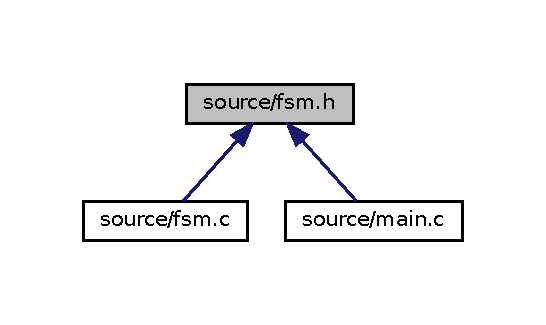
\includegraphics[width=262pt]{fsm_8h__dep__incl}
\end{center}
\end{figure}
\subsection*{Macros}
\begin{DoxyCompactItemize}
\item 
\#define \hyperlink{fsm_8h_afb1a2f0d6c57fd6e0f5f19a8849db177}{F\+O\+R\+E\+A\+C\+H\+\_\+\+S\+T\+A\+TE}(S\+T\+A\+TE)
\begin{DoxyCompactList}\small\item\em All the states the elevator can be in. \end{DoxyCompactList}\item 
\#define \hyperlink{fsm_8h_a44c518a36b9b9e429f17c7f9b1a621e0}{F\+O\+R\+E\+A\+C\+H\+\_\+\+E\+V\+E\+NT}(E\+V\+E\+NT)
\begin{DoxyCompactList}\small\item\em All events recognized by the state machine. \end{DoxyCompactList}\item 
\#define \hyperlink{fsm_8h_aed8760364c7992625d06c93d12b2496d}{G\+E\+N\+E\+R\+A\+T\+E\+\_\+\+E\+N\+UM}(E\+N\+UM)~E\+N\+UM,
\item 
\#define \hyperlink{fsm_8h_adf58d994c35f18ec84b628d8321f52e5}{G\+E\+N\+E\+R\+A\+T\+E\+\_\+\+S\+T\+R\+I\+NG}(S\+T\+R\+I\+NG)~\#S\+T\+R\+I\+NG,
\end{DoxyCompactItemize}
\subsection*{Enumerations}
\begin{DoxyCompactItemize}
\item 
\mbox{\Hypertarget{fsm_8h_a493217321e8eec123f3a1a788dddcf11}\label{fsm_8h_a493217321e8eec123f3a1a788dddcf11}} 
enum {\bfseries fsm\+\_\+event\+\_\+t} 
\item 
\mbox{\Hypertarget{fsm_8h_aefd70b8b91d72cbd548b6c38f385983b}\label{fsm_8h_aefd70b8b91d72cbd548b6c38f385983b}} 
enum {\bfseries fsm\+\_\+state\+\_\+t} 
\end{DoxyCompactItemize}
\subsection*{Functions}
\begin{DoxyCompactItemize}
\item 
void \hyperlink{fsm_8h_a6d28dcad43166c03b061f129a8759018}{fsm\+\_\+init} ()
\begin{DoxyCompactList}\small\item\em Sets initial state of state machine. \end{DoxyCompactList}\item 
void \hyperlink{fsm_8h_ae32fa4506316ff022e43d7b7ca2d34b2}{fsm\+\_\+dispatch} (fsm\+\_\+event\+\_\+t event)
\begin{DoxyCompactList}\small\item\em Dispatches event to the state machine. \end{DoxyCompactList}\item 
fsm\+\_\+state\+\_\+t \hyperlink{fsm_8h_a5e2a31ca4d677528882e4654158b7b70}{fsm\+\_\+get\+\_\+state} ()
\begin{DoxyCompactList}\small\item\em Returns current state of state machine. \end{DoxyCompactList}\item 
int \hyperlink{fsm_8h_a6cd8cafb76b77cf609f4aec4978a4f60}{fsm\+\_\+get\+\_\+floor} ()
\begin{DoxyCompactList}\small\item\em Retruns current floor of elevator. \end{DoxyCompactList}\end{DoxyCompactItemize}


\subsection{Detailed Description}
Finite state machine for an elevator. 

\begin{DoxyNote}{Note}
Based on \href{https://barrgroup.com/embedded-systems/how-to/state-machines-event-driven-systems}{\tt https\+://barrgroup.\+com/embedded-\/systems/how-\/to/state-\/machines-\/event-\/driven-\/systems} 
\end{DoxyNote}


\subsection{Macro Definition Documentation}
\mbox{\Hypertarget{fsm_8h_a44c518a36b9b9e429f17c7f9b1a621e0}\label{fsm_8h_a44c518a36b9b9e429f17c7f9b1a621e0}} 
\index{fsm.\+h@{fsm.\+h}!F\+O\+R\+E\+A\+C\+H\+\_\+\+E\+V\+E\+NT@{F\+O\+R\+E\+A\+C\+H\+\_\+\+E\+V\+E\+NT}}
\index{F\+O\+R\+E\+A\+C\+H\+\_\+\+E\+V\+E\+NT@{F\+O\+R\+E\+A\+C\+H\+\_\+\+E\+V\+E\+NT}!fsm.\+h@{fsm.\+h}}
\subsubsection{\texorpdfstring{F\+O\+R\+E\+A\+C\+H\+\_\+\+E\+V\+E\+NT}{FOREACH\_EVENT}}
{\footnotesize\ttfamily \#define F\+O\+R\+E\+A\+C\+H\+\_\+\+E\+V\+E\+NT(\begin{DoxyParamCaption}\item[{}]{E\+V\+E\+NT }\end{DoxyParamCaption})}

{\bfseries Value\+:}
\begin{DoxyCode}
EVENT(EVENT\_FLOOR\_1)                \(\backslash\)
        EVENT(EVENT\_FLOOR\_2)                \(\backslash\)
        EVENT(EVENT\_FLOOR\_3)                \(\backslash\)
        EVENT(EVENT\_FLOOR\_4)                \(\backslash\)
        EVENT(EVENT\_HW\_INIT\_DONE)           \(\backslash\)
        EVENT(EVENT\_STOP\_BUTTON\_PRESSED)    \(\backslash\)
        EVENT(EVENT\_STOP\_BUTTON\_RELEASED)   \(\backslash\)
        EVENT(EVENT\_TIMER\_TIMEOUT)          \(\backslash\)
        EVENT(EVENT\_OBSTRUCTION\_ACTIVE)     \(\backslash\)
        EVENT(EVENT\_QUEUE\_NOT\_EMPTY)        \(\backslash\)
        EVENT(EVENT\_ENTRY)                  \(\backslash\)
        EVENT(EVENT\_EXIT)
\end{DoxyCode}


All events recognized by the state machine. 

\begin{DoxyNote}{Note}
E\+V\+E\+N\+T\+\_\+\+F\+L\+O\+O\+R1-\/4 placed in beginning to use numerical value 

E\+V\+E\+N\+T\+\_\+\+E\+N\+T\+RY and E\+V\+E\+N\+T\+\_\+\+E\+X\+IT for internal F\+SM use only 
\end{DoxyNote}


Definition at line 30 of file fsm.\+h.

\mbox{\Hypertarget{fsm_8h_afb1a2f0d6c57fd6e0f5f19a8849db177}\label{fsm_8h_afb1a2f0d6c57fd6e0f5f19a8849db177}} 
\index{fsm.\+h@{fsm.\+h}!F\+O\+R\+E\+A\+C\+H\+\_\+\+S\+T\+A\+TE@{F\+O\+R\+E\+A\+C\+H\+\_\+\+S\+T\+A\+TE}}
\index{F\+O\+R\+E\+A\+C\+H\+\_\+\+S\+T\+A\+TE@{F\+O\+R\+E\+A\+C\+H\+\_\+\+S\+T\+A\+TE}!fsm.\+h@{fsm.\+h}}
\subsubsection{\texorpdfstring{F\+O\+R\+E\+A\+C\+H\+\_\+\+S\+T\+A\+TE}{FOREACH\_STATE}}
{\footnotesize\ttfamily \#define F\+O\+R\+E\+A\+C\+H\+\_\+\+S\+T\+A\+TE(\begin{DoxyParamCaption}\item[{}]{S\+T\+A\+TE }\end{DoxyParamCaption})}

{\bfseries Value\+:}
\begin{DoxyCode}
STATE(STATE\_INIT)                   \(\backslash\)
        STATE(STATE\_UNKNOWN\_FLOOR)          \(\backslash\)
        STATE(STATE\_IDLE)                   \(\backslash\)
        STATE(STATE\_MOVING)                 \(\backslash\)
        STATE(STATE\_DOOR\_OPEN)              \(\backslash\)
        STATE(STATE\_EMERGENCY\_STOP)         \(\backslash\)
        STATE(STATE\_EMERGENCY\_STOP\_FLOOR)   \(\backslash\)
        STATE(STATE\_EMERGENCY\_STOP\_NOWHERE)
\end{DoxyCode}


All the states the elevator can be in. 



Definition at line 14 of file fsm.\+h.

\mbox{\Hypertarget{fsm_8h_aed8760364c7992625d06c93d12b2496d}\label{fsm_8h_aed8760364c7992625d06c93d12b2496d}} 
\index{fsm.\+h@{fsm.\+h}!G\+E\+N\+E\+R\+A\+T\+E\+\_\+\+E\+N\+UM@{G\+E\+N\+E\+R\+A\+T\+E\+\_\+\+E\+N\+UM}}
\index{G\+E\+N\+E\+R\+A\+T\+E\+\_\+\+E\+N\+UM@{G\+E\+N\+E\+R\+A\+T\+E\+\_\+\+E\+N\+UM}!fsm.\+h@{fsm.\+h}}
\subsubsection{\texorpdfstring{G\+E\+N\+E\+R\+A\+T\+E\+\_\+\+E\+N\+UM}{GENERATE\_ENUM}}
{\footnotesize\ttfamily \#define G\+E\+N\+E\+R\+A\+T\+E\+\_\+\+E\+N\+UM(\begin{DoxyParamCaption}\item[{}]{E\+N\+UM }\end{DoxyParamCaption})~E\+N\+UM,}

Generates enumerated values 

Definition at line 45 of file fsm.\+h.

\mbox{\Hypertarget{fsm_8h_adf58d994c35f18ec84b628d8321f52e5}\label{fsm_8h_adf58d994c35f18ec84b628d8321f52e5}} 
\index{fsm.\+h@{fsm.\+h}!G\+E\+N\+E\+R\+A\+T\+E\+\_\+\+S\+T\+R\+I\+NG@{G\+E\+N\+E\+R\+A\+T\+E\+\_\+\+S\+T\+R\+I\+NG}}
\index{G\+E\+N\+E\+R\+A\+T\+E\+\_\+\+S\+T\+R\+I\+NG@{G\+E\+N\+E\+R\+A\+T\+E\+\_\+\+S\+T\+R\+I\+NG}!fsm.\+h@{fsm.\+h}}
\subsubsection{\texorpdfstring{G\+E\+N\+E\+R\+A\+T\+E\+\_\+\+S\+T\+R\+I\+NG}{GENERATE\_STRING}}
{\footnotesize\ttfamily \#define G\+E\+N\+E\+R\+A\+T\+E\+\_\+\+S\+T\+R\+I\+NG(\begin{DoxyParamCaption}\item[{}]{S\+T\+R\+I\+NG }\end{DoxyParamCaption})~\#S\+T\+R\+I\+NG,}

Generates stringified values 

Definition at line 48 of file fsm.\+h.



\subsection{Function Documentation}
\mbox{\Hypertarget{fsm_8h_ae32fa4506316ff022e43d7b7ca2d34b2}\label{fsm_8h_ae32fa4506316ff022e43d7b7ca2d34b2}} 
\index{fsm.\+h@{fsm.\+h}!fsm\+\_\+dispatch@{fsm\+\_\+dispatch}}
\index{fsm\+\_\+dispatch@{fsm\+\_\+dispatch}!fsm.\+h@{fsm.\+h}}
\subsubsection{\texorpdfstring{fsm\+\_\+dispatch()}{fsm\_dispatch()}}
{\footnotesize\ttfamily void fsm\+\_\+dispatch (\begin{DoxyParamCaption}\item[{fsm\+\_\+event\+\_\+t}]{event }\end{DoxyParamCaption})}



Dispatches event to the state machine. 


\begin{DoxyParams}{Parameters}
{\em event} & The event to be handled by the state machine \\
\hline
\end{DoxyParams}


Definition at line 66 of file fsm.\+c.

\mbox{\Hypertarget{fsm_8h_a6cd8cafb76b77cf609f4aec4978a4f60}\label{fsm_8h_a6cd8cafb76b77cf609f4aec4978a4f60}} 
\index{fsm.\+h@{fsm.\+h}!fsm\+\_\+get\+\_\+floor@{fsm\+\_\+get\+\_\+floor}}
\index{fsm\+\_\+get\+\_\+floor@{fsm\+\_\+get\+\_\+floor}!fsm.\+h@{fsm.\+h}}
\subsubsection{\texorpdfstring{fsm\+\_\+get\+\_\+floor()}{fsm\_get\_floor()}}
{\footnotesize\ttfamily int fsm\+\_\+get\+\_\+floor (\begin{DoxyParamCaption}{ }\end{DoxyParamCaption})}



Retruns current floor of elevator. 

\begin{DoxyReturn}{Returns}
int floor number, 0 indexed 
\end{DoxyReturn}


Definition at line 77 of file fsm.\+c.

\mbox{\Hypertarget{fsm_8h_a5e2a31ca4d677528882e4654158b7b70}\label{fsm_8h_a5e2a31ca4d677528882e4654158b7b70}} 
\index{fsm.\+h@{fsm.\+h}!fsm\+\_\+get\+\_\+state@{fsm\+\_\+get\+\_\+state}}
\index{fsm\+\_\+get\+\_\+state@{fsm\+\_\+get\+\_\+state}!fsm.\+h@{fsm.\+h}}
\subsubsection{\texorpdfstring{fsm\+\_\+get\+\_\+state()}{fsm\_get\_state()}}
{\footnotesize\ttfamily fsm\+\_\+state\+\_\+t fsm\+\_\+get\+\_\+state (\begin{DoxyParamCaption}{ }\end{DoxyParamCaption})}



Returns current state of state machine. 

\begin{DoxyReturn}{Returns}
fsm\+\_\+state\+\_\+t The current state of the state machine 
\end{DoxyReturn}


Definition at line 72 of file fsm.\+c.

\mbox{\Hypertarget{fsm_8h_a6d28dcad43166c03b061f129a8759018}\label{fsm_8h_a6d28dcad43166c03b061f129a8759018}} 
\index{fsm.\+h@{fsm.\+h}!fsm\+\_\+init@{fsm\+\_\+init}}
\index{fsm\+\_\+init@{fsm\+\_\+init}!fsm.\+h@{fsm.\+h}}
\subsubsection{\texorpdfstring{fsm\+\_\+init()}{fsm\_init()}}
{\footnotesize\ttfamily void fsm\+\_\+init (\begin{DoxyParamCaption}{ }\end{DoxyParamCaption})}



Sets initial state of state machine. 

\begin{DoxyNote}{Note}
Should only be called once at startup of program 
\end{DoxyNote}


Definition at line 61 of file fsm.\+c.


\hypertarget{hardware_8h}{}\section{source/hardware.h File Reference}
\label{hardware_8h}\index{source/hardware.\+h@{source/hardware.\+h}}


Driver for the elevator hardware.  


This graph shows which files directly or indirectly include this file\+:
\nopagebreak
\begin{figure}[H]
\begin{center}
\leavevmode
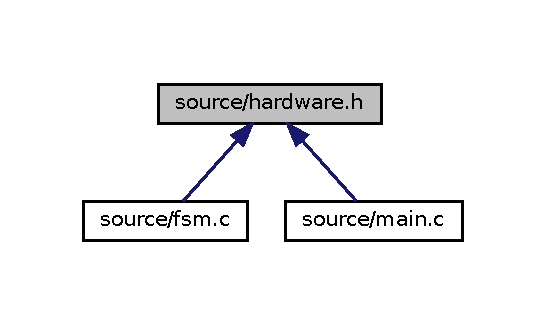
\includegraphics[width=262pt]{hardware_8h__dep__incl}
\end{center}
\end{figure}
\subsection*{Macros}
\begin{DoxyCompactItemize}
\item 
\mbox{\Hypertarget{hardware_8h_ae9e42615eade15633bd8c03b7a271a00}\label{hardware_8h_ae9e42615eade15633bd8c03b7a271a00}} 
\#define {\bfseries H\+A\+R\+D\+W\+A\+R\+E\+\_\+\+N\+U\+M\+B\+E\+R\+\_\+\+O\+F\+\_\+\+F\+L\+O\+O\+RS}~4
\item 
\mbox{\Hypertarget{hardware_8h_a966cbacea011640db5803364bff5ed53}\label{hardware_8h_a966cbacea011640db5803364bff5ed53}} 
\#define {\bfseries H\+A\+R\+D\+W\+A\+R\+E\+\_\+\+N\+U\+M\+B\+E\+R\+\_\+\+O\+F\+\_\+\+B\+U\+T\+T\+O\+NS}~3
\end{DoxyCompactItemize}
\subsection*{Enumerations}
\begin{DoxyCompactItemize}
\item 
\mbox{\Hypertarget{hardware_8h_a2167c399a24df296afc432bcb88228af}\label{hardware_8h_a2167c399a24df296afc432bcb88228af}} 
enum \hyperlink{hardware_8h_a2167c399a24df296afc432bcb88228af}{Hardware\+Movement} \{ {\bfseries H\+A\+R\+D\+W\+A\+R\+E\+\_\+\+M\+O\+V\+E\+M\+E\+N\+T\+\_\+\+UP}, 
{\bfseries H\+A\+R\+D\+W\+A\+R\+E\+\_\+\+M\+O\+V\+E\+M\+E\+N\+T\+\_\+\+S\+T\+OP}, 
{\bfseries H\+A\+R\+D\+W\+A\+R\+E\+\_\+\+M\+O\+V\+E\+M\+E\+N\+T\+\_\+\+D\+O\+WN}
 \}\begin{DoxyCompactList}\small\item\em Movement type used in {\ttfamily hardware\+\_\+command\+\_\+movement}. \end{DoxyCompactList}
\item 
\mbox{\Hypertarget{hardware_8h_a796a8de8ce0ae769d7dbd3327a7bdbe7}\label{hardware_8h_a796a8de8ce0ae769d7dbd3327a7bdbe7}} 
enum \hyperlink{hardware_8h_a796a8de8ce0ae769d7dbd3327a7bdbe7}{Hardware\+Order} \{ {\bfseries H\+A\+R\+D\+W\+A\+R\+E\+\_\+\+O\+R\+D\+E\+R\+\_\+\+UP}, 
{\bfseries H\+A\+R\+D\+W\+A\+R\+E\+\_\+\+O\+R\+D\+E\+R\+\_\+\+I\+N\+S\+I\+DE}, 
{\bfseries H\+A\+R\+D\+W\+A\+R\+E\+\_\+\+O\+R\+D\+E\+R\+\_\+\+D\+O\+WN}
 \}\begin{DoxyCompactList}\small\item\em Order type used in {\ttfamily hardware\+\_\+read\+\_\+order} and in {\ttfamily hardware\+\_\+command\+\_\+order\+\_\+light}. \end{DoxyCompactList}
\end{DoxyCompactItemize}
\subsection*{Functions}
\begin{DoxyCompactItemize}
\item 
int \hyperlink{hardware_8h_a054b8fb8768311d46be58d6a4890d771}{hardware\+\_\+init} ()
\begin{DoxyCompactList}\small\item\em Initializes the elevator control hardware. Must be called once before other calls to the elevator hardware driver. \end{DoxyCompactList}\item 
void \hyperlink{hardware_8h_a01de081ef0510a111053c18cd31afa27}{hardware\+\_\+command\+\_\+movement} (\hyperlink{hardware_8h_a2167c399a24df296afc432bcb88228af}{Hardware\+Movement} movement)
\begin{DoxyCompactList}\small\item\em Commands the elevator to either move up or down, or commands it to halt. \end{DoxyCompactList}\item 
int \hyperlink{hardware_8h_a4a77b27c86675c00b513db3445966804}{hardware\+\_\+read\+\_\+stop\+\_\+signal} ()
\begin{DoxyCompactList}\small\item\em Polls the hardware for the current stop signal. \end{DoxyCompactList}\item 
int \hyperlink{hardware_8h_a459fe57a3ee4bc2a28e8a15b2ab14c2d}{hardware\+\_\+read\+\_\+obstruction\+\_\+signal} ()
\begin{DoxyCompactList}\small\item\em Polls the hardware for the current obstruction signal. \end{DoxyCompactList}\item 
int \hyperlink{hardware_8h_ab048489e6302bb5604aad753f2d7d501}{hardware\+\_\+read\+\_\+floor\+\_\+sensor} (int floor)
\begin{DoxyCompactList}\small\item\em Polls the floor sensor for the given {\ttfamily floor}. \end{DoxyCompactList}\item 
int \hyperlink{hardware_8h_a87917f3aa093fb46ca821a400d011ee8}{hardware\+\_\+read\+\_\+order} (int floor, \hyperlink{hardware_8h_a796a8de8ce0ae769d7dbd3327a7bdbe7}{Hardware\+Order} order\+\_\+type)
\begin{DoxyCompactList}\small\item\em Polls the hardware for the status of orders from floor {\ttfamily floor} of type {\ttfamily order\+\_\+type}. \end{DoxyCompactList}\item 
void \hyperlink{hardware_8h_a80d99ddaa8e7b58c9a88b60ea553c1b6}{hardware\+\_\+command\+\_\+door\+\_\+open} (int door\+\_\+open)
\begin{DoxyCompactList}\small\item\em Commands the hardware to open-\/ or close the elevator door. \end{DoxyCompactList}\item 
void \hyperlink{hardware_8h_a407a6ec035ba357de6aa0fbe55501d1e}{hardware\+\_\+command\+\_\+floor\+\_\+indicator\+\_\+on} (int floor)
\begin{DoxyCompactList}\small\item\em Commands the hardware to turn on the floor indicator for {\ttfamily floor}. All indicators all mutually exclusive; other indicator lights will turn off. \end{DoxyCompactList}\item 
void \hyperlink{hardware_8h_aa75b3ac17f72b25946414f48d0063a10}{hardware\+\_\+command\+\_\+stop\+\_\+light} (int on)
\begin{DoxyCompactList}\small\item\em Sets the light in the panel stop button. \end{DoxyCompactList}\item 
void \hyperlink{hardware_8h_aa9b33faa52f0ec5b614d3e7dc05be140}{hardware\+\_\+command\+\_\+order\+\_\+light} (int floor, \hyperlink{hardware_8h_a796a8de8ce0ae769d7dbd3327a7bdbe7}{Hardware\+Order} order\+\_\+type, int on)
\begin{DoxyCompactList}\small\item\em Sets the light in a button corresponding to an order of type {\ttfamily order\+\_\+type}, at floor {\ttfamily floor}. \end{DoxyCompactList}\end{DoxyCompactItemize}


\subsection{Detailed Description}
Driver for the elevator hardware. 

Neatly wraps up Martin Korsgaard\textquotesingle{}s spaghetti from 2006 ;)

Kolbjørn Austreng 

\subsection{Function Documentation}
\mbox{\Hypertarget{hardware_8h_a80d99ddaa8e7b58c9a88b60ea553c1b6}\label{hardware_8h_a80d99ddaa8e7b58c9a88b60ea553c1b6}} 
\index{hardware.\+h@{hardware.\+h}!hardware\+\_\+command\+\_\+door\+\_\+open@{hardware\+\_\+command\+\_\+door\+\_\+open}}
\index{hardware\+\_\+command\+\_\+door\+\_\+open@{hardware\+\_\+command\+\_\+door\+\_\+open}!hardware.\+h@{hardware.\+h}}
\subsubsection{\texorpdfstring{hardware\+\_\+command\+\_\+door\+\_\+open()}{hardware\_command\_door\_open()}}
{\footnotesize\ttfamily void hardware\+\_\+command\+\_\+door\+\_\+open (\begin{DoxyParamCaption}\item[{int}]{door\+\_\+open }\end{DoxyParamCaption})}



Commands the hardware to open-\/ or close the elevator door. 


\begin{DoxyParams}{Parameters}
{\em door\+\_\+open} & A truthy value (non-\/zero) to open the door; 0 to close. \\
\hline
\end{DoxyParams}
\mbox{\Hypertarget{hardware_8h_a407a6ec035ba357de6aa0fbe55501d1e}\label{hardware_8h_a407a6ec035ba357de6aa0fbe55501d1e}} 
\index{hardware.\+h@{hardware.\+h}!hardware\+\_\+command\+\_\+floor\+\_\+indicator\+\_\+on@{hardware\+\_\+command\+\_\+floor\+\_\+indicator\+\_\+on}}
\index{hardware\+\_\+command\+\_\+floor\+\_\+indicator\+\_\+on@{hardware\+\_\+command\+\_\+floor\+\_\+indicator\+\_\+on}!hardware.\+h@{hardware.\+h}}
\subsubsection{\texorpdfstring{hardware\+\_\+command\+\_\+floor\+\_\+indicator\+\_\+on()}{hardware\_command\_floor\_indicator\_on()}}
{\footnotesize\ttfamily void hardware\+\_\+command\+\_\+floor\+\_\+indicator\+\_\+on (\begin{DoxyParamCaption}\item[{int}]{floor }\end{DoxyParamCaption})}



Commands the hardware to turn on the floor indicator for {\ttfamily floor}. All indicators all mutually exclusive; other indicator lights will turn off. 


\begin{DoxyParams}{Parameters}
{\em floor} & Floor to turn on the indicator for.\\
\hline
\end{DoxyParams}
\begin{DoxyWarning}{Warning}
Owing to peculiarities in the hardware construction, there will always be one indicator active. 
\end{DoxyWarning}
\mbox{\Hypertarget{hardware_8h_a01de081ef0510a111053c18cd31afa27}\label{hardware_8h_a01de081ef0510a111053c18cd31afa27}} 
\index{hardware.\+h@{hardware.\+h}!hardware\+\_\+command\+\_\+movement@{hardware\+\_\+command\+\_\+movement}}
\index{hardware\+\_\+command\+\_\+movement@{hardware\+\_\+command\+\_\+movement}!hardware.\+h@{hardware.\+h}}
\subsubsection{\texorpdfstring{hardware\+\_\+command\+\_\+movement()}{hardware\_command\_movement()}}
{\footnotesize\ttfamily void hardware\+\_\+command\+\_\+movement (\begin{DoxyParamCaption}\item[{\hyperlink{hardware_8h_a2167c399a24df296afc432bcb88228af}{Hardware\+Movement}}]{movement }\end{DoxyParamCaption})}



Commands the elevator to either move up or down, or commands it to halt. 


\begin{DoxyParams}{Parameters}
{\em movement} & Commanded movement. \\
\hline
\end{DoxyParams}
\mbox{\Hypertarget{hardware_8h_aa9b33faa52f0ec5b614d3e7dc05be140}\label{hardware_8h_aa9b33faa52f0ec5b614d3e7dc05be140}} 
\index{hardware.\+h@{hardware.\+h}!hardware\+\_\+command\+\_\+order\+\_\+light@{hardware\+\_\+command\+\_\+order\+\_\+light}}
\index{hardware\+\_\+command\+\_\+order\+\_\+light@{hardware\+\_\+command\+\_\+order\+\_\+light}!hardware.\+h@{hardware.\+h}}
\subsubsection{\texorpdfstring{hardware\+\_\+command\+\_\+order\+\_\+light()}{hardware\_command\_order\_light()}}
{\footnotesize\ttfamily void hardware\+\_\+command\+\_\+order\+\_\+light (\begin{DoxyParamCaption}\item[{int}]{floor,  }\item[{\hyperlink{hardware_8h_a796a8de8ce0ae769d7dbd3327a7bdbe7}{Hardware\+Order}}]{order\+\_\+type,  }\item[{int}]{on }\end{DoxyParamCaption})}



Sets the light in a button corresponding to an order of type {\ttfamily order\+\_\+type}, at floor {\ttfamily floor}. 


\begin{DoxyParams}{Parameters}
{\em floor} & The floor of the order indicator. \\
\hline
{\em order\+\_\+type} & The type of order. \\
\hline
{\em on} & A truthy value (non-\/zero) to turn the light on; 0 to turn it off. \\
\hline
\end{DoxyParams}
\mbox{\Hypertarget{hardware_8h_aa75b3ac17f72b25946414f48d0063a10}\label{hardware_8h_aa75b3ac17f72b25946414f48d0063a10}} 
\index{hardware.\+h@{hardware.\+h}!hardware\+\_\+command\+\_\+stop\+\_\+light@{hardware\+\_\+command\+\_\+stop\+\_\+light}}
\index{hardware\+\_\+command\+\_\+stop\+\_\+light@{hardware\+\_\+command\+\_\+stop\+\_\+light}!hardware.\+h@{hardware.\+h}}
\subsubsection{\texorpdfstring{hardware\+\_\+command\+\_\+stop\+\_\+light()}{hardware\_command\_stop\_light()}}
{\footnotesize\ttfamily void hardware\+\_\+command\+\_\+stop\+\_\+light (\begin{DoxyParamCaption}\item[{int}]{on }\end{DoxyParamCaption})}



Sets the light in the panel stop button. 


\begin{DoxyParams}{Parameters}
{\em on} & A truthy value (non-\/zero) to turn the light on; 0 to turn it off. \\
\hline
\end{DoxyParams}
\mbox{\Hypertarget{hardware_8h_a054b8fb8768311d46be58d6a4890d771}\label{hardware_8h_a054b8fb8768311d46be58d6a4890d771}} 
\index{hardware.\+h@{hardware.\+h}!hardware\+\_\+init@{hardware\+\_\+init}}
\index{hardware\+\_\+init@{hardware\+\_\+init}!hardware.\+h@{hardware.\+h}}
\subsubsection{\texorpdfstring{hardware\+\_\+init()}{hardware\_init()}}
{\footnotesize\ttfamily int hardware\+\_\+init (\begin{DoxyParamCaption}{ }\end{DoxyParamCaption})}



Initializes the elevator control hardware. Must be called once before other calls to the elevator hardware driver. 

\begin{DoxyReturn}{Returns}
0 on success. Non-\/zero for failure. 
\end{DoxyReturn}
\mbox{\Hypertarget{hardware_8h_ab048489e6302bb5604aad753f2d7d501}\label{hardware_8h_ab048489e6302bb5604aad753f2d7d501}} 
\index{hardware.\+h@{hardware.\+h}!hardware\+\_\+read\+\_\+floor\+\_\+sensor@{hardware\+\_\+read\+\_\+floor\+\_\+sensor}}
\index{hardware\+\_\+read\+\_\+floor\+\_\+sensor@{hardware\+\_\+read\+\_\+floor\+\_\+sensor}!hardware.\+h@{hardware.\+h}}
\subsubsection{\texorpdfstring{hardware\+\_\+read\+\_\+floor\+\_\+sensor()}{hardware\_read\_floor\_sensor()}}
{\footnotesize\ttfamily int hardware\+\_\+read\+\_\+floor\+\_\+sensor (\begin{DoxyParamCaption}\item[{int}]{floor }\end{DoxyParamCaption})}



Polls the floor sensor for the given {\ttfamily floor}. 


\begin{DoxyParams}{Parameters}
{\em floor} & Inquired floor.\\
\hline
\end{DoxyParams}
\begin{DoxyReturn}{Returns}
1 if the elevator is at {\ttfamily floor}, otherwise 0; 
\end{DoxyReturn}
\mbox{\Hypertarget{hardware_8h_a459fe57a3ee4bc2a28e8a15b2ab14c2d}\label{hardware_8h_a459fe57a3ee4bc2a28e8a15b2ab14c2d}} 
\index{hardware.\+h@{hardware.\+h}!hardware\+\_\+read\+\_\+obstruction\+\_\+signal@{hardware\+\_\+read\+\_\+obstruction\+\_\+signal}}
\index{hardware\+\_\+read\+\_\+obstruction\+\_\+signal@{hardware\+\_\+read\+\_\+obstruction\+\_\+signal}!hardware.\+h@{hardware.\+h}}
\subsubsection{\texorpdfstring{hardware\+\_\+read\+\_\+obstruction\+\_\+signal()}{hardware\_read\_obstruction\_signal()}}
{\footnotesize\ttfamily int hardware\+\_\+read\+\_\+obstruction\+\_\+signal (\begin{DoxyParamCaption}{ }\end{DoxyParamCaption})}



Polls the hardware for the current obstruction signal. 

\begin{DoxyReturn}{Returns}
1 if the obstruction signal is high; 0 if it is low. 
\end{DoxyReturn}
\mbox{\Hypertarget{hardware_8h_a87917f3aa093fb46ca821a400d011ee8}\label{hardware_8h_a87917f3aa093fb46ca821a400d011ee8}} 
\index{hardware.\+h@{hardware.\+h}!hardware\+\_\+read\+\_\+order@{hardware\+\_\+read\+\_\+order}}
\index{hardware\+\_\+read\+\_\+order@{hardware\+\_\+read\+\_\+order}!hardware.\+h@{hardware.\+h}}
\subsubsection{\texorpdfstring{hardware\+\_\+read\+\_\+order()}{hardware\_read\_order()}}
{\footnotesize\ttfamily int hardware\+\_\+read\+\_\+order (\begin{DoxyParamCaption}\item[{int}]{floor,  }\item[{\hyperlink{hardware_8h_a796a8de8ce0ae769d7dbd3327a7bdbe7}{Hardware\+Order}}]{order\+\_\+type }\end{DoxyParamCaption})}



Polls the hardware for the status of orders from floor {\ttfamily floor} of type {\ttfamily order\+\_\+type}. 


\begin{DoxyParams}{Parameters}
{\em floor} & Inquired floor. \\
\hline
{\em order\+\_\+type} & \\
\hline
\end{DoxyParams}
\begin{DoxyReturn}{Returns}
1 if the combination of {\ttfamily floor} and {\ttfamily order\+\_\+type} is being requested, otherwise 0. 
\end{DoxyReturn}
\mbox{\Hypertarget{hardware_8h_a4a77b27c86675c00b513db3445966804}\label{hardware_8h_a4a77b27c86675c00b513db3445966804}} 
\index{hardware.\+h@{hardware.\+h}!hardware\+\_\+read\+\_\+stop\+\_\+signal@{hardware\+\_\+read\+\_\+stop\+\_\+signal}}
\index{hardware\+\_\+read\+\_\+stop\+\_\+signal@{hardware\+\_\+read\+\_\+stop\+\_\+signal}!hardware.\+h@{hardware.\+h}}
\subsubsection{\texorpdfstring{hardware\+\_\+read\+\_\+stop\+\_\+signal()}{hardware\_read\_stop\_signal()}}
{\footnotesize\ttfamily int hardware\+\_\+read\+\_\+stop\+\_\+signal (\begin{DoxyParamCaption}{ }\end{DoxyParamCaption})}



Polls the hardware for the current stop signal. 

\begin{DoxyReturn}{Returns}
1 if the stop signal is high; 0 if it is low. 
\end{DoxyReturn}

\hypertarget{queue_8h}{}\section{source/queue.h File Reference}
\label{queue_8h}\index{source/queue.\+h@{source/queue.\+h}}


Elevator queue implementation.  


This graph shows which files directly or indirectly include this file\+:
\nopagebreak
\begin{figure}[H]
\begin{center}
\leavevmode
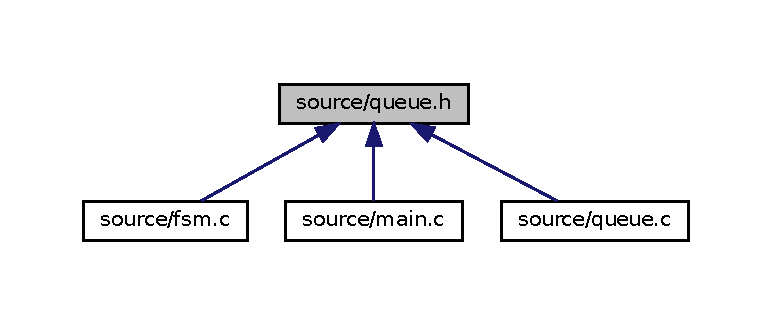
\includegraphics[width=350pt]{queue_8h__dep__incl}
\end{center}
\end{figure}
\subsection*{Macros}
\begin{DoxyCompactItemize}
\item 
\#define \hyperlink{queue_8h_a8b928421e9bb547953b629579d455bca}{Q\+U\+E\+U\+E\+\_\+\+E\+M\+P\+TY}~-\/1
\end{DoxyCompactItemize}
\subsection*{Enumerations}
\begin{DoxyCompactItemize}
\item 
\mbox{\Hypertarget{queue_8h_ae9ae980041e438eed7a3af43ce4e9f6b}\label{queue_8h_ae9ae980041e438eed7a3af43ce4e9f6b}} 
enum {\bfseries direction\+\_\+t} \{ {\bfseries D\+I\+R\+E\+C\+T\+I\+O\+N\+\_\+\+UP}, 
{\bfseries D\+I\+R\+E\+C\+T\+I\+O\+N\+\_\+\+D\+O\+WN}
 \}
\end{DoxyCompactItemize}
\subsection*{Functions}
\begin{DoxyCompactItemize}
\item 
void \hyperlink{queue_8h_acc09874bb09dfc3f053a9df4ac13ab4c}{queue\+\_\+add\+\_\+request} (int floor, direction\+\_\+t requested\+\_\+direction)
\begin{DoxyCompactList}\small\item\em Adds a request to the queue. \end{DoxyCompactList}\item 
void \hyperlink{queue_8h_a26b3b217e3f5df5aaf55a8d345e081df}{queue\+\_\+remove\+\_\+request} (int floor, direction\+\_\+t requested\+\_\+direction)
\begin{DoxyCompactList}\small\item\em Removes a fulfilled request from the queue. \end{DoxyCompactList}\item 
void \hyperlink{queue_8h_ab89a10c9e2068760936a23d782ec12a6}{queue\+\_\+get\+\_\+next} (int current\+\_\+floor, direction\+\_\+t moving\+\_\+direction, int $\ast$next\+\_\+floor, direction\+\_\+t $\ast$next\+\_\+direction)
\begin{DoxyCompactList}\small\item\em Retrieves the next element in the queue to travel to. \end{DoxyCompactList}\item 
\mbox{\Hypertarget{queue_8h_adb8d2b079d228f27e2d4dbb71ff48de0}\label{queue_8h_adb8d2b079d228f27e2d4dbb71ff48de0}} 
void \hyperlink{queue_8h_adb8d2b079d228f27e2d4dbb71ff48de0}{queue\+\_\+clear} ()
\begin{DoxyCompactList}\small\item\em Erases all requests in queue. \end{DoxyCompactList}\end{DoxyCompactItemize}


\subsection{Detailed Description}
Elevator queue implementation. 



\subsection{Macro Definition Documentation}
\mbox{\Hypertarget{queue_8h_a8b928421e9bb547953b629579d455bca}\label{queue_8h_a8b928421e9bb547953b629579d455bca}} 
\index{queue.\+h@{queue.\+h}!Q\+U\+E\+U\+E\+\_\+\+E\+M\+P\+TY@{Q\+U\+E\+U\+E\+\_\+\+E\+M\+P\+TY}}
\index{Q\+U\+E\+U\+E\+\_\+\+E\+M\+P\+TY@{Q\+U\+E\+U\+E\+\_\+\+E\+M\+P\+TY}!queue.\+h@{queue.\+h}}
\subsubsection{\texorpdfstring{Q\+U\+E\+U\+E\+\_\+\+E\+M\+P\+TY}{QUEUE\_EMPTY}}
{\footnotesize\ttfamily \#define Q\+U\+E\+U\+E\+\_\+\+E\+M\+P\+TY~-\/1}

Value used for signaling that the queue is empty 

Definition at line 9 of file queue.\+h.



\subsection{Function Documentation}
\mbox{\Hypertarget{queue_8h_acc09874bb09dfc3f053a9df4ac13ab4c}\label{queue_8h_acc09874bb09dfc3f053a9df4ac13ab4c}} 
\index{queue.\+h@{queue.\+h}!queue\+\_\+add\+\_\+request@{queue\+\_\+add\+\_\+request}}
\index{queue\+\_\+add\+\_\+request@{queue\+\_\+add\+\_\+request}!queue.\+h@{queue.\+h}}
\subsubsection{\texorpdfstring{queue\+\_\+add\+\_\+request()}{queue\_add\_request()}}
{\footnotesize\ttfamily void queue\+\_\+add\+\_\+request (\begin{DoxyParamCaption}\item[{int}]{floor,  }\item[{direction\+\_\+t}]{requested\+\_\+direction }\end{DoxyParamCaption})}



Adds a request to the queue. 


\begin{DoxyParams}{Parameters}
{\em floor} & Floor to travel to. 0 indexed, \char`\"{}\+Floor 1\char`\"{} is 0 \\
\hline
{\em requested\+\_\+direction} & Requested direction of travel \\
\hline
\end{DoxyParams}


Definition at line 10 of file queue.\+c.

\mbox{\Hypertarget{queue_8h_ab89a10c9e2068760936a23d782ec12a6}\label{queue_8h_ab89a10c9e2068760936a23d782ec12a6}} 
\index{queue.\+h@{queue.\+h}!queue\+\_\+get\+\_\+next@{queue\+\_\+get\+\_\+next}}
\index{queue\+\_\+get\+\_\+next@{queue\+\_\+get\+\_\+next}!queue.\+h@{queue.\+h}}
\subsubsection{\texorpdfstring{queue\+\_\+get\+\_\+next()}{queue\_get\_next()}}
{\footnotesize\ttfamily void queue\+\_\+get\+\_\+next (\begin{DoxyParamCaption}\item[{int}]{current\+\_\+floor,  }\item[{direction\+\_\+t}]{moving\+\_\+direction,  }\item[{int $\ast$}]{next\+\_\+floor,  }\item[{direction\+\_\+t $\ast$}]{next\+\_\+direction }\end{DoxyParamCaption})}



Retrieves the next element in the queue to travel to. 


\begin{DoxyParams}{Parameters}
{\em current\+\_\+floor} & The current floor the elevator is in \\
\hline
{\em moving\+\_\+direction} & The current direction of travel for the elevator \\
\hline
{\em next\+\_\+floor} & \mbox{[}out\mbox{]} The next floor to travel to, set to Q\+U\+E\+U\+E\+\_\+\+E\+M\+P\+TY if nothing in queue \\
\hline
{\em moving\+\_\+direction} & \mbox{[}out\mbox{]} The requested direction, not updated if nothing in queue\\
\hline
\end{DoxyParams}
\begin{DoxyWarning}{Warning}
Providing N\+U\+LL pointers to {\ttfamily next\+\_\+floor} or {\ttfamily moving\+\_\+direction} will lead to badness 
\end{DoxyWarning}


Definition at line 34 of file queue.\+c.

\mbox{\Hypertarget{queue_8h_a26b3b217e3f5df5aaf55a8d345e081df}\label{queue_8h_a26b3b217e3f5df5aaf55a8d345e081df}} 
\index{queue.\+h@{queue.\+h}!queue\+\_\+remove\+\_\+request@{queue\+\_\+remove\+\_\+request}}
\index{queue\+\_\+remove\+\_\+request@{queue\+\_\+remove\+\_\+request}!queue.\+h@{queue.\+h}}
\subsubsection{\texorpdfstring{queue\+\_\+remove\+\_\+request()}{queue\_remove\_request()}}
{\footnotesize\ttfamily void queue\+\_\+remove\+\_\+request (\begin{DoxyParamCaption}\item[{int}]{floor,  }\item[{direction\+\_\+t}]{requested\+\_\+direction }\end{DoxyParamCaption})}



Removes a fulfilled request from the queue. 


\begin{DoxyParams}{Parameters}
{\em floor} & Current floor \\
\hline
{\em requested\+\_\+direction} & Current direction \\
\hline
\end{DoxyParams}


Definition at line 22 of file queue.\+c.


\hypertarget{timer_8h}{}\section{source/timer.h File Reference}
\label{timer_8h}\index{source/timer.\+h@{source/timer.\+h}}


Implements a timer that times out in {\ttfamily T\+I\+M\+E\+R\+\_\+\+T\+I\+M\+E\+O\+U\+T\+\_\+\+S\+E\+C\+O\+N\+DS} seconds.  


{\ttfamily \#include $<$stdbool.\+h$>$}\newline
Include dependency graph for timer.\+h\+:
\nopagebreak
\begin{figure}[H]
\begin{center}
\leavevmode
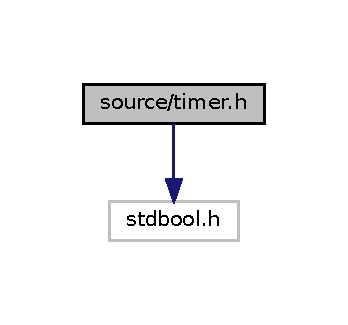
\includegraphics[width=167pt]{timer_8h__incl}
\end{center}
\end{figure}
This graph shows which files directly or indirectly include this file\+:
\nopagebreak
\begin{figure}[H]
\begin{center}
\leavevmode
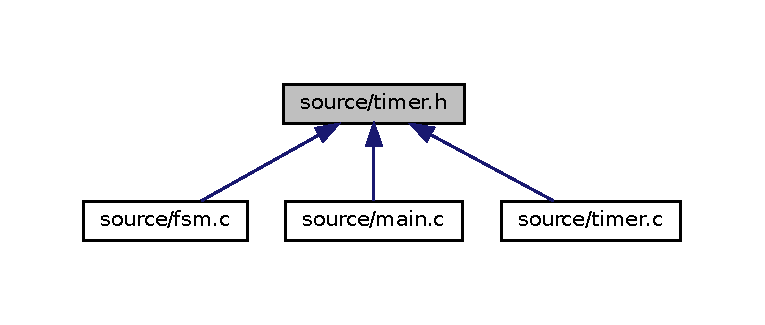
\includegraphics[width=350pt]{timer_8h__dep__incl}
\end{center}
\end{figure}
\subsection*{Macros}
\begin{DoxyCompactItemize}
\item 
\mbox{\Hypertarget{timer_8h_a6ad8f18a9074717b11bb80d5e874c890}\label{timer_8h_a6ad8f18a9074717b11bb80d5e874c890}} 
\#define {\bfseries T\+I\+M\+E\+R\+\_\+\+T\+I\+M\+O\+U\+T\+\_\+\+S\+E\+C\+O\+N\+DS}~3
\end{DoxyCompactItemize}
\subsection*{Functions}
\begin{DoxyCompactItemize}
\item 
\mbox{\Hypertarget{timer_8h_ab0af1c6dfc5bcd5292a73401ff223b75}\label{timer_8h_ab0af1c6dfc5bcd5292a73401ff223b75}} 
void \hyperlink{timer_8h_ab0af1c6dfc5bcd5292a73401ff223b75}{timer\+\_\+restart} ()
\begin{DoxyCompactList}\small\item\em Saves current unix timestamp. \end{DoxyCompactList}\item 
bool \hyperlink{timer_8h_a0fc45745263e4aef123b9851e7ab4120}{timer\+\_\+check\+\_\+timeout} ()
\begin{DoxyCompactList}\small\item\em Checks if timer has timed out. \end{DoxyCompactList}\end{DoxyCompactItemize}


\subsection{Detailed Description}
Implements a timer that times out in {\ttfamily T\+I\+M\+E\+R\+\_\+\+T\+I\+M\+E\+O\+U\+T\+\_\+\+S\+E\+C\+O\+N\+DS} seconds. 



\subsection{Function Documentation}
\mbox{\Hypertarget{timer_8h_a0fc45745263e4aef123b9851e7ab4120}\label{timer_8h_a0fc45745263e4aef123b9851e7ab4120}} 
\index{timer.\+h@{timer.\+h}!timer\+\_\+check\+\_\+timeout@{timer\+\_\+check\+\_\+timeout}}
\index{timer\+\_\+check\+\_\+timeout@{timer\+\_\+check\+\_\+timeout}!timer.\+h@{timer.\+h}}
\subsubsection{\texorpdfstring{timer\+\_\+check\+\_\+timeout()}{timer\_check\_timeout()}}
{\footnotesize\ttfamily bool timer\+\_\+check\+\_\+timeout (\begin{DoxyParamCaption}{ }\end{DoxyParamCaption})}



Checks if timer has timed out. 

\begin{DoxyReturn}{Returns}
true More than {\ttfamily T\+I\+M\+E\+R\+\_\+\+T\+I\+M\+E\+O\+U\+T\+\_\+\+S\+E\+C\+O\+N\+DS} seconds since last call to \hyperlink{timer_8h_ab0af1c6dfc5bcd5292a73401ff223b75}{timer\+\_\+restart()} 

false Otherwise
\end{DoxyReturn}
\begin{DoxyWarning}{Warning}
\hyperlink{timer_8h_ab0af1c6dfc5bcd5292a73401ff223b75}{timer\+\_\+restart()} should be called at least once to get known behaviour 
\end{DoxyWarning}


Definition at line 14 of file timer.\+c.


%--- End generated contents ---

% Index
\backmatter
\newpage
\phantomsection
\clearemptydoublepage
\addcontentsline{toc}{chapter}{Index}
\printindex

\end{document}
